\chapter{Il bridge}
\label{cha:bridge}

\section{Generalità e piccola digressione sul MUX}
\label{sec:generalitaDMAC}

Il DMA Controller fornisce un meccanismo d'accelerazione per il trasferimento dei dati fra la RAM e la periferica; il suo scopo è quello di fungere da co-processore di supporto, assumendo di tanto in tanto il ruolo di \textit{master} del bus, alleggerendo la CPU e diminuendo drasticamente il numero di interrupt che quest'ultima deve gestire. La presenza contemporanea di CPU e DMAC rende la nostra architettura già \textit{multiprocessor}, almeno a livello concettuale.

\subsection{Il MUX e altri animali}

\begin{figure}[!h]
\centering
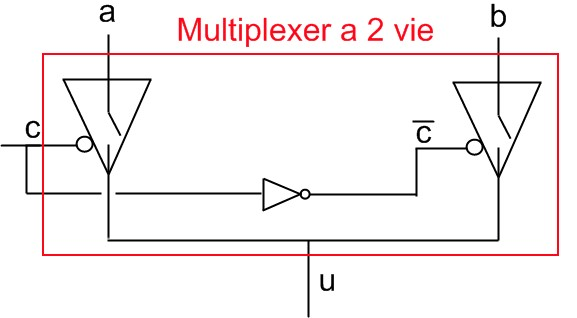
\includegraphics[width=0.58743626456\columnwidth]{img/mux2vie}
\caption{Radiografia di un multiplexer a 2 vie}
\label{fig:mux2vie}
\end{figure}

In figura \ref{fig:mux2vie} vediamo schematicamente l'interno di un semplicissimo multiplexer a 2 vie\footnote{Notiamo la presenza del fondamentale componente \textit{Buffer 3-state} e di un gate NOT.}:
\[
u=a \bar c + bc
\]
In figura \ref{fig:mux4vie} i vediamo invece la struttura di un multiplexer a 4 vie costruito mediante un decoder 2:4 (che ci dà la sicurezza di avere un'unica via attivata).

\begin{figure}[!h]
\centering
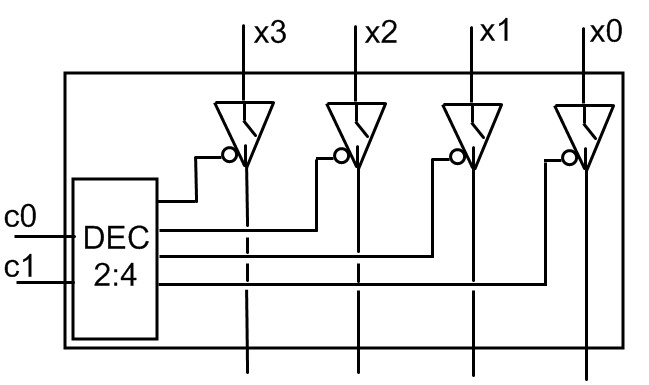
\includegraphics[width=0.57676586356213452354687654324567876543\columnwidth]{img/mux4vie}
\caption{Radiografia di un multiplexer a 4 vie}
\label{fig:mux4vie}
\end{figure}

\section{Bridge e sua struttura}
\label{sec:bridgeStruttura}

Se al posto dei buffer ora mettiamo i componenti 244 ("'batterie'" di 8 buffer divise in due gruppi da 4, attivate dagli \textit{output enable }OE0 ed OE1, vedi fig. \ref{fig:244}) siamo già sulla buona strada per creare una delle due direzioni del nostro \textit{bridge}: in parole povere esso funziona come un multiplexer a 8 vie, solo che invece si convogliare i singoli bit si convogliano blocchi da 8 bit (vedi fig. \ref{fig:briggiu}).

\begin{figure}[!h]
\centering
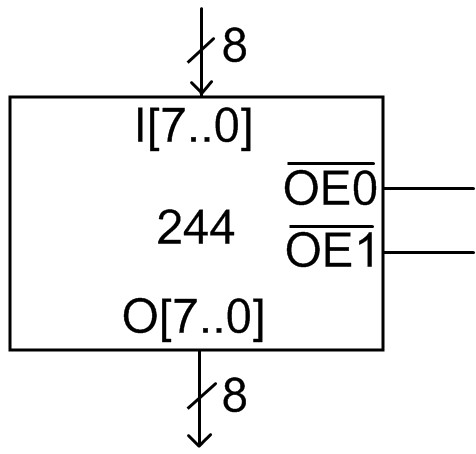
\includegraphics[width=0.35\columnwidth]{img/244}
\caption{Il componente 244}
\label{fig:244}
\end{figure}

\begin{figure}[!h]
\centering
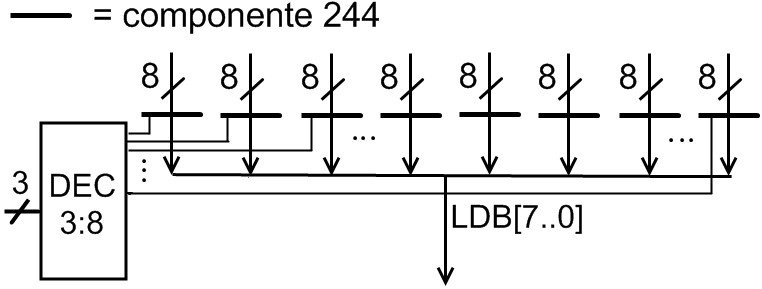
\includegraphics[width=0.75\columnwidth]{img/briggiu}
\caption{Bridge: dalla memoria alle periferiche}
\label{fig:briggiu}
\end{figure}

Al decoder in figura \ref{fig:briggiu} arrivano i tre bit generati dall'encoder che prende in pasto gli 8 segnali di \textit{bank enable} (vedi capitolo \ref{cha:centralMem}): a questo punto qualcuno potrebbe obiettare che non ha senso mettere un decoder a valle di un encoder, tuttavia è opportuno che siano presenti entrambi in quanto c'è il rischio che non vi sia sempre un unico segnale di \textit{bank enable} attivo, cosa che potrebbe portare ad un conflitto elettrico all'interno del MUX. Il nostro scopo è invece quello di svincolare il microprocessore dal doversi preoccupare dei conflitti del multiplexer\footnote{Magari chi ha scritto il software era uno stolto!}, per cui rinunceremo al risparmio che otterremmo nel rimuovere la cascata encoder + decoder.

Problema: stanti così le cose, il bus di I/O rischia di essere contemporaneamente pilotato sia dalla periferica che da i driver 244. Anche questo potrebbe essere causa di conflitto elettrico, dunque dobbiamo tirare in ballo qualche segnale di controllo (IORD*, IOWR*, MEMRD*, MEMWR*)\footnote{La dicitura potrebbe cambiare, nel corso della trattazione: si potrà ad esempio trovare IO/MEM*, W/R*, MRDC*, IOWC*, etc\ldots Stiamo comunque parlando degli stessi segnali, l'importante è sapersi intendere!} per segnalare se la CPU sta leggendo (RD) o scrivendo (WR) in memoria (MEM) o da/verso le periferiche (IO). Se ad esempio stiamo scrivendo sulla periferica sarà necessario abilitare il bridge tramite l'abbassamento del segnale IOWR*. Risulta inoltre intuitivo il fatto che il DMAC, effettuando trasferimenti fra la periferica e la memoria, dovrà in tali frangenti attivare contemporaneamente MEMWR* e IORD*.

Sarà inoltre necessario contemplare uno schema come quello in figura \ref{fig:briggiu}, che "'salga'" verso le memorie compiendo il percorso inverso rispetto a quello visto poco fa. Nella sostanza nulla cambia, basta girare le frecce: l'unico punto delicato consiste nella scelta dei segnali di \textit{output enable } per i 244 che portano al bus della memoria. In questo caso non c'è bisogno di un decoder per pilotarli: possiamo anzi attivarli tutti contemporaneamente (quando leggiamo dalla periferica), tanto poi il microprocessore aggiornerà soltanto il banco coinvolto in quel particolare ciclo di bus e in quella particolare transazione (gli altri manco li degna di attenzione!).
Quel che non deve accadere è che vi siano conflitti fra la lettura e la scrittura, quindi dovremo oportunamente collegare i segnali MEM/IO* e WR/RD* agli \textit{output enable} di cui sopra: in questo modo il nostro multiplexer si spegnerà quando non ci sarà bisogno di lui, con un conseguente risparmio anche in termini energetici e, allo stesso tempo, eviteremo l'eventuale conflitto che si potrebbe avere quando il microprocessore va a leggere in memoria e attiva RD* (se non vi fosse MEM/IO* il bridge si attiverebbe senza motivo, visto che leggiamo in memoria e non nella periferica).

Se siamo sadici e preferiamo interfacciare la nostra periferica direttamente al bus dati\footnote{Scelta sconsigliata!} (piuttosto che sfruttare il bridge), dobbiamo avere cura di predisporre un segnale che disabiliti il bridge quando leggiamo da quella determinata periferica: in caso contrario vi sarebbe un conflitto elettrico fra il "'sopra'" (memoria, CPU e a questo punto anche la nostra periferica) e il "'sotto'" (DMAC, PIC, altre periferiche, etc\ldots) del nostro famoso schema (riportato anche in figura \ref{fig:schemaSolito}). Tutto questo comporta un complicarsi della logica di controllo e richiede maggiore attenzione in sede di progetto.

Regola generale è comunque la seguente: se interfaccio il dispositivo in memoria userò indirizzi \textit{interleaved}, mentre se collego la periferica al bus di I/O gli indirizzi saranno contigui.

\begin{figure}[!h]
\centering
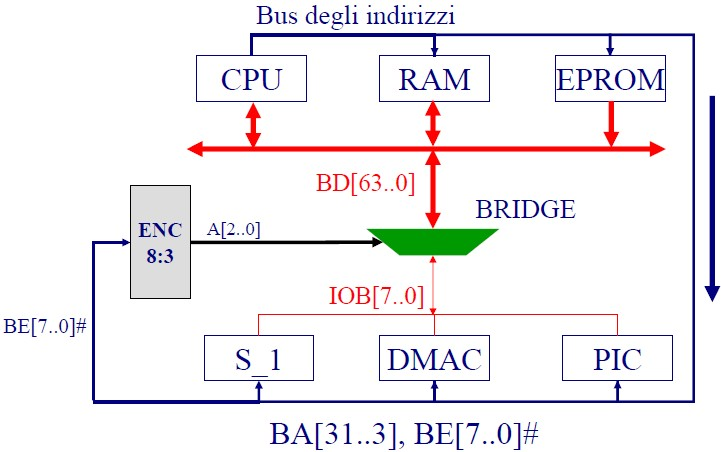
\includegraphics[width=0.75\columnwidth]{img/schemaSolito}
\caption{Struttura del calcolatore (in sitesi)}
\label{fig:schemaSolito}
\end{figure}

In figura \ref{fig:ciclivari} vengono graficate alcune forme d'onda rappresentanti i segnali che qualificano il ciclo di bus: se M/IO* è vero e W/R* è negato significa che stiamo leggendo dalla memoria (è l'equivalente del segnale MEMRD*, chiamato MRDC* in figura); se, viceversa, M/IO* è negato e W/R* è vero significa che stiamo scrivendo in memoria (IOWRC* attivato), ad esempio perché stiamo effettuando un'operazione di OUT. Si noti che c'è bisogno di rispettare un tempo di \textit{set-up} e di \textit{hold} perché il dato sia valido. 

\begin{figure}[!h]
\centering
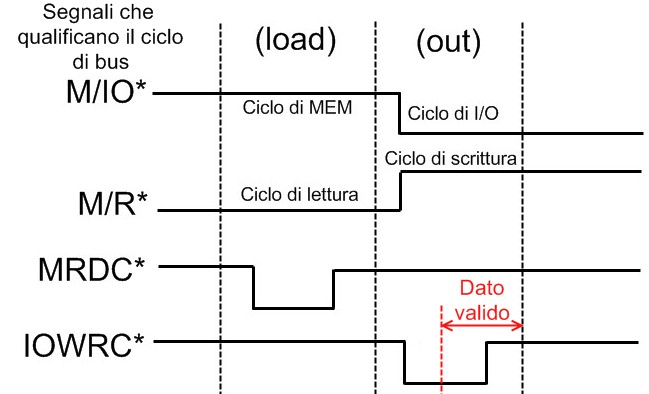
\includegraphics[width=0.6\columnwidth]{img/ciclivari}
\caption{Segnali che qualificano il ciclo di bus}
\label{fig:ciclivari}
\end{figure}

Qualificare il ciclo di bus è importante non solo per gli ovvi motivi riguardanti il bridge e i conflitti elettrici, ma anche perché in base a cosa dovremo fare avremo un ciclo di bus specifico fissato da una macchina a stati (vedi fig. \ref{fig:macchinaStatiCicloBus}.

\begin{figure}[!h]
\centering
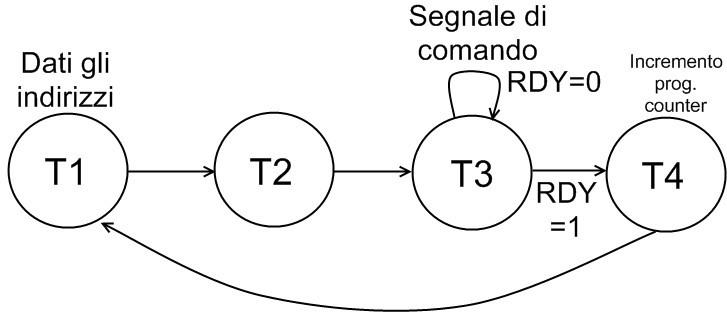
\includegraphics[width=0.65\columnwidth]{img/macchinaStatiCicloBus}
\caption{Macchina a stati che regola il ciclo di bus}
\label{fig:macchinaStatiCicloBus}
\end{figure}

\section{Bridge bidirezionale}
\label{sec:bridgeBidi}

Se utilizziamo dei componenti 245 siamo in grado di creare un \textit{bridge bidirezionale} che sappia sfruttare i segnali di qualificazione del ciclo di bus per una gestione ottimale del dispositivo. Due sono le vie che è possibile seguire (e tre gli stati possibili):
\begin{itemize}
\item "'verso l'alto'", cioè dalle periferiche alla memoria (chiameremo questo caso \textit{ricezione});
\item "'verso il basso'", cioè dalla memoria alle periferiche (chiameremo questo caso \textit{trasmissione});
\item in alternativa a queste opzioni è possibile spegnere completamente il dispositivo (non dobbiamo far nulla).
\end{itemize}
Per gestire queste tre eventualità servono i segnali di controllo:
\begin{itemize}
\item T/R*, di trasmissione/ricezione;
\item OE*, di \textit{output enable}, che indica se vogliamo fare qualcosa oppure no.
\end{itemize}

\begin{figure}[!h]
\centering
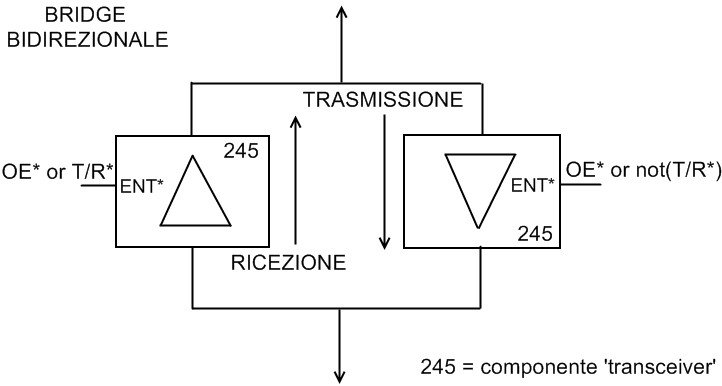
\includegraphics[width=0.55\columnwidth]{img/bridgeBidirezionale}
\caption{Bridge bidirezionale costruito con componenti 245}
\label{fig:bridgeBidirezionale}
\end{figure}

A cosa colleghiamo T/R* e OE*?
T/R* sarà l'OR fra il segnale IORD* (che da solo non basterebbe, in quanto li PIC potrebbe intervenire quando più gli aggrada e confliggere) e INTA*. OE* lo colleghiamo invece al segnale M/IO*, tanto il bridge dev'essere non attivo tutte le volte che il microprocessore va in memoria e non sta andando in IO.
